\documentclass[12pt, leqno]{article} %% use to set typesize
\usepackage{fancyhdr}
\usepackage[sort&compress]{natbib}
\usepackage[letterpaper=true,colorlinks=true,linkcolor=black]{hyperref}

\usepackage{amsfonts}
\usepackage{amsmath}
\usepackage{amssymb}
\usepackage{color}
\usepackage{tikz}
\usepackage{pgfplots}
\usepackage{listings}
%\usepackage{courier}
%\usepackage[utf8]{inputenc}
%\usepackage[russian]{babel}

\lstset{
  numbers=left,
  basicstyle=\ttfamily\footnotesize,
  numberstyle=\tiny\color{gray},
  stepnumber=1,
  numbersep=10pt,
}

\newcommand{\iu}{\ensuremath{\mathrm{i}}}
\newcommand{\bbR}{\mathbb{R}}
\newcommand{\bbC}{\mathbb{C}}
\newcommand{\calV}{\mathcal{V}}
\newcommand{\calW}{\mathcal{W}}
\newcommand{\macheps}{\epsilon_{\mathrm{mach}}}
\newcommand{\matlab}{\textsc{Matlab}}

\newcommand{\ddiag}{\operatorname{diag}}
\newcommand{\fl}{\operatorname{fl}}
\newcommand{\nnz}{\operatorname{nnz}}
\newcommand{\tr}{\operatorname{tr}}
\renewcommand{\vec}{\operatorname{vec}}

\newcommand{\vertiii}[1]{{\left\vert\kern-0.25ex\left\vert\kern-0.25ex\left\vert #1
    \right\vert\kern-0.25ex\right\vert\kern-0.25ex\right\vert}}
\newcommand{\ip}[2]{\langle #1, #2 \rangle}
\newcommand{\ipx}[2]{\left\langle #1, #2 \right\rangle}
\newcommand{\order}[1]{O( #1 )}

\newcommand{\kron}{\otimes}


\newcommand{\hdr}[1]{
  \pagestyle{fancy}
  \lhead{Bindel, Summer 2018}
  \rhead{Numerics for Data Science}
  \fancyfoot{}
  \begin{center}
    {\large{\bf #1}}
  \end{center}
  \lstset{language=matlab,columns=flexible}  
}


\begin{document}
\hdr{2018-06-11}

\section{Introduction}

The title of this course is ``Numerical Methods for Data Science.''
What does that mean?  Before we dive into the course technical
material, let's put things into context.  I will not attempt to
completely define either ``numerical methods'' or ``data science,''
but will at least give some thoughts on each.

{\em Numerical methods} are algorithms that solve problems of
continuous mathematics: finding solutions to systems of linear or
nonlinear equations, minimizing or maximizing functions, computing
approximations to functions, simulating how systems of differential
equations evolve in time, and so forth.  Numerical methods are used
everywhere, and many mathematicians and scientists focus on designing
these methods, analyzing their properties, adapting them to work well
for specific types of problems, and implementing them to run fast on
modern computers.  Scientific computing, also called Computational
Science and Engineering (CSE), is about applying numerical methods ---
as well as the algorithms and approaches of discrete mathematics ---
to solve ``real world'' problems from some application field.
Though different researchers in scientific computing focus on different
aspects, they share the interplay between the domain expertise and
modeling, mathematical analysis, and efficient computation.

I have read many descriptions of {\em data science}, and have not been
satisfied by any of them.
The fashion now is to call oneself a data
scientist and (if in a university) perhaps to start a master's program
to train students to call themselves data scientists.  There are books
and web sites and conferences devoted to data science; SIAM even has a new
journal on the Mathematics of Data Science\footnote{%
  And I'll be excited to read the first issues!
}.
But what is data science, really?
Statisticians
may claim that data science is a modern rebranding of statistics.
Computer scientists may reply that it is all about machine
learning\footnote{The statisticians could retort that machine learning
  is itself a modern rebranding of statistics, with some
  justification.} and scalable algorithms for large data sets.
Experts from various scientific fields might claim the name of data
science for work that combines statistics, novel algorithms, and new
sources of large scale data like modern telescopes or DNA sequencers.
And from my biased perspective, data science sounds a lot like scientific computing!

Though I am uncertain how data science should be defined, I am certain
that a foundation of numerical methods should be involved.  Moreover,
I am certain that advances in data science, broadly construed, will
drive research in numerical method design in new and interesting
directions.  In this course, we will explore some of the fundamental
numerical methods for optimization, numerical linear algebra, and
function approximation, and see the role they play in different styles of
data analysis problems that are currently in fashion.  In particular,
we will spend one week each talking about
\begin{itemize}
\item Optimization methods for ML.
\item Latent factor models, factorizations, and analysis of
  matrix data.
\item Function approximation and kernel methods.
\item Numerical methods for graph data analysis.
\end{itemize}
You will not need to have a prior numerical analysis course for this
course, but you should have a good grounding in calculus and linear
algebra.  I have posted some
\href{http://www.cs.cornell.edu/~bindel/class/sjtu-summer18/lec/background.pdf}{background
  notes}
to remind you of some things you may have forgotten, and perhaps to
fill in some things you may not have seen.  Please do ask questions as
we go, and if you see anything that you think should be corrected or
clarified, send me an email (or you can suggest a change on the
\href{https://github.com/dbindel/sjtu-summer2018/}{course GitHub repository}).

\section{Optimization}

Much of this class\footnote{%
  There are also some topics in the class that do not fit naturally
  into an optimization framework, and we will deal with them as they come.
} will involve different types of optimization problems:
\begin{equation}
  \mbox{minimize } \phi(x) \mbox{ s.t. } x \in \Omega.
\end{equation}
Here $\phi : \bbR^n \rightarrow \bbR$ is the {\em objective function} and 
$\Omega$ is the {\em constraint set}, usually defined in terms of a
collection of constraint equations and inequalities:
\[
\Omega = \{ x \in \bbR^n :
  c_i(x) = 0, i \in \mathcal{E} \mbox{ and }
  c_i(x) \leq 0, i \in \mathcal{I} \}.
\]
A point in $\Omega$ is called {\em feasible}; points outside
$\Omega$ are {\em infeasible}.  In many cases, we will be able to
solve {\em unconstrained} problems where $\Omega$ is the entire domain of
the function (in this case, all of $\bbR^n$), so that every point is
feasible.

\begin{figure}
  \begin{center}
  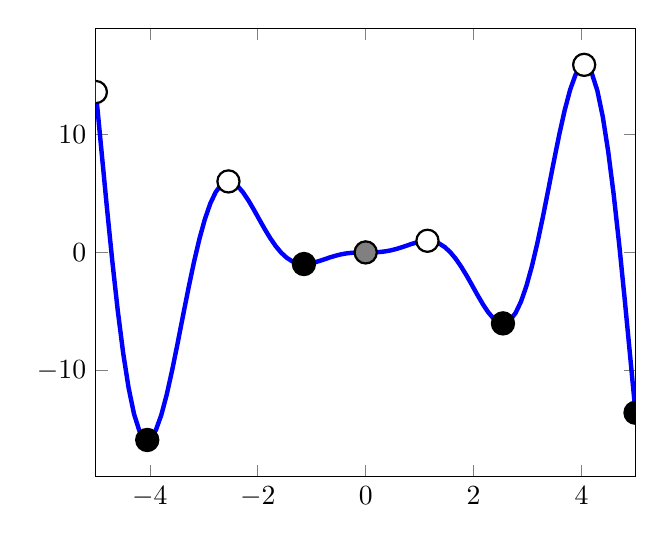
\begin{tikzpicture}
  \begin{axis}[xmin=-5,xmax=5]
    \addplot[domain=-5:5, samples=100, blue, ultra thick] (x,
            {x*x*(sin(deg(2*x)))});
    \filldraw [fill=black, thick] (axis cs:2.5435,-6.0207)
              circle [radius=4pt];
    \filldraw [fill=black, thick] (axis cs:-4.0481,-15.909)
              circle [radius=4pt];
    \filldraw [fill=black, thick] (axis cs:-1.1445,-0.98633)
              circle [radius=4pt];
    \filldraw [fill=black, thick] (axis cs:5,-13.601)
              circle [radius=4pt];
    \filldraw [fill=white, draw=black, thick] (axis cs:-2.5435,6.0207)
              circle [radius=4pt];
    \filldraw [fill=white, draw=black, thick] (axis cs:4.0481,15.909)
              circle [radius=4pt];
    \filldraw [fill=white, draw=black, thick] (axis cs:1.1445,0.98633)
              circle [radius=4pt];
    \filldraw [fill=white, draw=black, thick] (axis cs:-5,13.601)
              circle [radius=4pt];
    \filldraw [fill=black!50, draw=black, thick] (axis cs:0,0)
              circle [radius=4pt];
  \end{axis}
  \end{tikzpicture}
  \caption{The objective $\phi(x) = x^2 \sin(2x)$ on $\Omega = [-5,5]$
    has four local minima (black), along with four maxima (white) and
    one critical point which is neither (gray).  Most optimizers will
    only find one of the local minima, unless they are provided with
    a good initial guess at the global optimum.}
  \end{center}
\end{figure}

Even simple optimization problems need not have a solution.
For example, a function might not be bounded from below (e.g.~the
identity function $x \mapsto x$ on $\Omega = \bbR$), or there might
be an asymptotic lower bound that can never be achieved (e.g.~the
function $x \mapsto 1/x$ on $\Omega = \{ x \in \bbR : x > 0 \}$).
If $\phi$ is continuous and $\Omega$ is closed and bounded (i.e.~a
{\em compact} subset of $\bbR^n$), then at least there is some
$x_* \in \Omega$ that solves the global optimization problem problem:
that is, $\phi(x_*) \leq \phi(x)$ for all other $x \in \Omega$.
But just because a solution exists does not mean it is easy to
compute!  If all we know is that $\phi$ is continuous and $\Omega$ is
compact, any algorithm that provably converges to the global minimizer
must eventually sample densely in $\Omega$\footnote{%
  See {\em Global optimization} by T{\"o}rn and {\v{Z}}ilinskas.
}.  This statement of gloom
is usually too pessimistic, because we generally know more properties
than simple continuity of $\phi$.  Nonetheless, in many cases,
it may be too expensive to solve the global optimization
problem, or at least to prove that we have solved the problem.
In these cases, the best we know how to do in practices is to find a
good {\em local} minimizer, that is, a point $x_* \in \Omega$ such that
$\phi(x_*) \leq \phi(x)$ for all $x \in \Omega$ close enough to $x_*$.
If the inequality is strict, we call $x_*$ a {\em strong} local
minimizer.

The picture is rosier when we want to solve a {\em convex} problem; that is,
\begin{enumerate}
\item The {\em set} $\Omega$ is convex: $\forall x, y \in \Omega$, 
  we have $\alpha x + (1-\alpha) y \in \Omega$ for $0 < \alpha < 1$.
\item The {\em function} $\phi$ is convex on $\Omega$:
  for any $x, y \in \Omega$ and $0 < \alpha < 1$,
  \[
    \phi\left( \alpha x + (1-\alpha) y\right) \leq
    \alpha \phi(x) + (1-\alpha) \phi(y).
  \]
  If the inequality is strict, we say $\phi$ is {\em strongly} convex.
\end{enumerate}
For a convex problem, every local minimizer is also a global
minimizer, and the local minimizers (if there is more than one) form a
convex set.  If the function $\phi$ is strongly convex, then there is
only one minimizer for the problem.  Moreover, we have simple
algorithms that we can prove converge to the solution of a strongly
convex problem, though we might still decide we are unhappy about the
cost of these methods for large problems.

Whether or not they are convex, many of the optimization problems that
arise in machine learning and data science have special structure,
and we can take advantage of this structure when we develop
algorithms.  For example:
\begin{itemize}
\item
  Among the simplest and most widely used optimization problems
  are {\em linear programs}, where
  \[
    \phi(x) = c^T x
  \]
  subject to constraints $Ax \leq b$ and $x \geq 0$.  Among their many
  other uses, linear programs are a building block for
  {\em sparse recovery} methods in which we seek to represent a signal
  vector as a linear combination of a small number of elements in some
  dictionary set.  We will not discuss sparse recovery in detail, but
  will touch on it when we discuss {\em matrix completion} next week.

\item
  Unconstrained problems with {\em quadratic} objective functions
  \[
    \phi(x) = \frac{1}{2} x^T A x + b^T x + c
  \]
  are another simple and useful type.  A common special case is the
  {\em linear least squares} objective
  \[
    \phi(x) = \frac{1}{2} \|Ax-b\|^2
    = \frac{1}{2} x^T A^T A x - b^T Ax + \frac{1}{2} b^T b.
  \]
  We constantly optimize quadratic functions, both because they are
  useful on their own and because optimization of quadratics is a
  standard building block for more complicated problems.  Optimizing
  a quadratic objective is the same as solving a linear system, and
  so we can bring to bear many methods of modern linear algebra when
  solving this problem.  For example, a particularly popular approach
  is the {\em conjugate gradient} method.

\item
  In many cases, the objective is a sum of simple terms:
  \[
    \phi(x) = \sum_{i=1}^n \phi_i(x).
  \]
  An important case is the {\em nonlinear least squares} problem
  $\phi(x) = \|f(x)\|^2$, which we will discuss later this week.
  In modern machine learning, problems of this form are often solved
  by various {\em stochastic gradient} methods.
  
\item
  Most {\em spectral} methods in data science can be phrased in
  terms of the {\em quadratically constrained quadratic program}
  \[
    \phi(x) = \frac{1}{2} x^T A x + b^T x + c, \quad
    \Omega = \{ x \in \bbR^n : x^T M x = 1 \}.
  \]
  We will see such problems in matrix data analysis and also graph
  clustering and partitioning methods.  We can sometimes create methods
  for these problems that build on the fact that we have good methods
  for solving eigenvalue problems.

\item
  Some nonconvex objectives are {\em bi-convex}:
  $\phi(x_1, x_2)$ is a convex function of $x_1$ for a fixed
  $x_2$ and vice-versa, though not in $x$ as a whole.
  We will see these types of problems repeatedly
  when we consider analysis of matrix data.  We can sometimes create
  methods for these problems based on the idea of
  {\em block coordinate descent} (also known as {\em nonlinear Gauss-Seidel}
  or {\em alternating iterations}) that solve a sequence of convex
  subproblems in each of the variables in turn.

\item
  We also consider problems where
  $\phi$ (and possibly $\Omega$) depend on an additional parameter
  $s$; for example, in an optimization problem coming from regression,
  we might have an additional {\em regularization parameter}.  In this
  case, we might consider {\em continuation} methods that 
  compute the curve of solutions.
  
\end{itemize}

\section{Optimality conditions}

In an unconstrained problem with a differentiable objective
function, a necessary (but not sufficient) condition for $x_*$
to be a local minimizer is that $\phi'(x_*) = 0$.
For intuition, picture a function $\phi : \bbR^n \rightarrow \bbR$; if
you'd like to be concrete, let $n = 2$.  Absent a computer, we might
optimize $\phi$ by the physical experiment of dropping a tiny ball
onto the surface and watching it roll downhill (in the steepest
descent direction) until it reaches the minimum.  The statement
that $\phi'(x_*) = 0$ (or that $\nabla \phi(x_*) = 0$) basically means
the function looks flat at $x_*$ to a sufficiently near-sighted observer;
if $\phi'(x_*)$ is not zero, then $x_* - \epsilon \nabla \phi(x_*)$
will be a little bit ``downhill'' of $x_*$; that is,
if $\|\nabla \phi(x_*)\| \neq 0$ then
\[
  \phi(x_* - \epsilon \nabla \phi(x_*)) =
  \phi(x_*) - \epsilon \|\nabla \phi(x_*)\|^2 + o(\epsilon) < \phi(x_*)
\]
for sufficiently small $\epsilon$.

Most students learn the first-order optimality conditions for unconstrained
optimization in a first course, but sometimes that course gets
everyone too stuck on the idea of computing a gradient.  What is
really happening is that the function should be ``flat in all directions,''
i.e.~all directional derivatives are zero.  This is equivalent to the
statement that the gradient is zero, of course, but sometimes it is
notationally easier to check that an arbitrary directional derivative
is zero than to try to write down the gradient.  For example, consider
the quadratic objective
\[
  \phi(x) = \frac{1}{2} x^T A x + x^T b + c.
\]
Now, we will write an arbitrary directional derivative of $\phi$ in
terms of ``variational notation'' (described in the background notes):
\[
\delta \phi(x) =
\left. \frac{d}{d\epsilon} \right|_{\epsilon = 0} \phi(x+ \epsilon \delta x)
= (\delta x)^T (Ax + b).
\]
At a critical point, $\delta \phi(x)$ should be zero for any
choice of $\delta x$, so the stationary point occurs at $Ax_* + b = 0$.
There is a unique minimizer $x_*$ if $A$ is positive definite.
When the number of variables is not too large --- up to a few
thousand, say --- we might solve this system of linear equations
directly using a variant of Gaussian elimination
if we wanted to find the minimizer.  When the number of variables
is much larger, we may prefer to use an iterative method 
to solve the system, e.g.~the method of conjugate gradients (CG).
This method can be interpreted either as an iterative solver for
linear equations or as an iterative optimization method.

Now let's turn to the {\em constrained} case.  Rather than repeating
the formal derivation of the first-order constrained optimality
conditions that you have likely seen before, let me again give you an
interpretation that involves some physical intuition.  For the
unconstrained case, we thought about solving the problem by rolling
a tiny ball down hill until it came to rest.  If we wanted to solve a
constrained minimization problem, we could build a great wall between
the feasible and the infeasible region.  A ball rolling into the wall
would still roll freely in directions tangent to the wall (or away
from the wall) if those directions were downhill; at a constrained
miminizer, the force pulling the ball downhill would be perfectly
balanced against an opposing force pushing into the feasible region
in the direction of the normal to the wall.  If the feasible region
is $\{x : c(x) \leq 0\}$, the normal direction pointing inward at a
boundary point $x_*$ s.t.~$c(x_*) = 0$ is proportional to
$-\nabla c(x_*)$.  Hence, if $x_*$ is a constrained minimum,
we expect the sum of the ``rolling downhill'' force ($-\nabla \phi$)
and something proportional to $-\nabla c(x_*)$ to be zero:
\[
  -\nabla \phi(x_*) - \mu \nabla c(x_*) = 0.
\]
The {\em Lagrange multiplier} $\mu$ in this picture represents the
magnitude of the restoring force from the wall balancing the tendency
to roll downhill.

More abstractly, and more generally, suppose that we have a mix of
equality and inequality constraints.  We define
the {\em augmented Lagrangian}
\[
  L(x, \lambda, \mu) = \phi(x) +
    \sum_{i \in \mathcal{E}} \lambda_i c_i(x) +
    \sum_{i \in \mathcal{I}} \mu_i c_i(x).
\]
The {\em Karush-Kuhn-Tucker (KKT) conditions} for $x_*$ to be a
constrained minimizer are
\begin{align*}
  \nabla_x L(x_*) &= 0 \\
  c_i(x_*) &= 0, \quad i \in \mathcal{E}
  & \mbox{equality constraints}\\
  c_i(x_*) & \leq 0, \quad i \in \mathcal{I}
  & \mbox{inequality constraints}\\
  \mu_i & \geq 0, \quad i \in \mathcal{I}
  & \mbox{non-negativity of multipliers}\\
  c_i(x_*) \mu_i &= 0, \quad i \in \mathcal{I}
  & \mbox{complementary slackness}
\end{align*}
where the (negative of) the ``total force'' at $x_*$ is
\[
  \nabla_x L(x_*) = \nabla \phi(x_*) +
    \sum_{i\in \mathcal{E}} \lambda_i \nabla c_i(x_*) +
    \sum_{i\in \mathcal{I}} \mu_i \nabla c_i(x_*).
\]
The complementary slackness condition corresponds to the idea that a
multiplier should be nonzero only if the corresponding constraint is
active (a ``restoring force'' is only present if our test ball
is pushed into a wall).

Like the critical point equation in the unconstrained case, the KKT
conditions define a set of (necessary but not sufficient) nonlinear
algebraic equations that must be satisfied at a minimizer.  I like to
think about the ``rolling downhill'' intuition for these necessary
conditions because it suggests a way of thinking about numerical
methods.

For completeness, we will say a few brief words about
the second-order {\em sufficient} conditions for optimality.
In the unconstrained case, $x_*$ is a strong
local minimizer of $\phi$ if $\nabla \phi(x_*) = 0$ and
the Hessian matrix $H_{\phi}$ is positive definite; that is because
in this case $x_*$ is the strong minimizer of the quadratic approximation
\[
  \phi(x) \approx \phi(x_*) + \frac{1}{2} (x-x_*)^T H_\phi(x_*) (x-x_*).
\]
In the constrained case, the Hessian only needs to be positive
definite for those $u$ that are orthogonal to $\nabla c_i(x_*)$
for each $c_i$ that is active (has a nonzero Lagrange multiplier).
We will see this idea in two weeks when we talk about kernel methods,
and in particular talk about the idea of
a {\em conditionally positive definite} kernel function.

\section{Numerical methods}

With our lightning review of some fundamental theory out of the way,
it is time to turn to numerical methods!  In particular, we will spend
the next three lectures talking about gradient and stochastic gradient
methods, Newton and Gauss-Newton, and (block) coordinate descent.
We will see additional solver ideas as we move through the semester,
but these are nicely prototypical examples that illustrate two running
themes in the design of numerical methods for optimization.

\paragraph{Fixed point iterations}
All our nonlinear solvers (and some of our linear solvers) will be
{\em iterative}.  We can write most as {\em fixed point iterations}
\begin{equation}
  x^{k+1} = G(x^k), \label{eq:fixed-point}
\end{equation}
which we hope will converge to a fixed point, i.e. $x^* = G(x^*)$.
We often approach convergence analysis through the
{\em error iteration} relating the error $e^k = x^k-x^*$ at
successive steps:
\begin{equation}
  e^{k+1} = G(x^* + e^k)-G(x^*).
\end{equation}

As a teaser for this sort of analysis, consider one of the simplest
algorithms I know: gradient descent with a fixed step size $h$, applied
to the quadratic model problem
\[
  \phi(x) = \frac{1}{2} x^T A x + b^T x + c
\]
where $A$ is assumed to be symmetric and positive definite.  The
algorithm produces iterates
\begin{align*}
  x^{k+1}
  &= x^k - h \nabla \phi(x^k) \\
  &= x^k - h (Ax^k + b) \\
  &= (I-hA) x^k - h b.
\end{align*}
Now we subtract the fixed point equation for the true solution $x^*$
in order to get an error iteration:
\begin{align*}
    & [x^{k+1} = (I-hA) x^k - hb] \\
  - & [x^*     = (I-hA) x^* - hb] \\ \hline
  = & [e^{k+1} = (I-hA) e^k ]
\end{align*}
where $e^k = x^k-x^*$.  The error iteration converges iff the largest
eigenvalue of $A$ is less than $2 h^{-1}$; if this condition is
satisfied, then
\[
  \|e^{k+1}\| \leq (1-h\lambda_{\max}(A)) \|e^k\|
\]
and so we have $\|e^{k+1}\| \leq (1-h\lambda_{\max}(A))^{k+1} \|e^0\|$,
a convergence rate which is known as (R)-linear convergence or
as geometric convergence, depending on which corner of the literature
one prefers to read.

\paragraph{Model-based methods}
Most nonquadratic problems are too hard to solve directly.  On the other
hand, we can {\em model} hard nonquadratic problems by simpler (possibly
linear) problems as a way of building iterative solvers.  The most
common tactic --- but not the only one! --- is to approximate the
nonlinear function by a linear or quadratic function and apply all the
things we know about linear algebra.  We will return to this idea in
the next lecture when we discuss Newton-type methods for optimization.


\end{document}
